\chapter{Morse functions on point clouds}

We now focus on discrete augmented metric spaces.
In particular, suppose we have a compact smooth manifold
$M$ equipped with a Morse function $f:M\to \mathbb{R}$.

From this manifold $M$ we sample a finite amount of points 
$X=\{x_i\}_{i=0}^n$ and we record the value of $f$ on $X$.

We investigate what sort of topological information we can recover from this
discrete sample.

The first thing we would like to do is recover the gradient of the function.
For this purpose we create a graph using $X$ as its base set
and we define a flow on the graph by moving from one point to the point
connected with it where the morse function $f$ takes the smallest value.

\begin{definition}[NNG graph]

Given $X$ a discrete set,
we define $G^-(X)$ it's descending pseudo-gradient graph
as the nearest neighbour graph of $X$. 

That is the graph where the 
edges $\{x_i,x_j\}$ are precisely where either $d(x_i,x_j)=d(x_i,X)$
or $d(x_i,x_j)=d(x_j,X)$. Notice that the binary relation $x_i\sim x_j$ if 
and only if
$x_j$ is the closest vertex to $x_i$ is not symmetric.

We denote as $\omega^-:G\to G$ the application that
maps $p\in X$ to the result of iteratively following the point
with that its joined to $p$ and that minimises the value of $f$.

We define $\alpha^-$ in an analogous manner, by following the direction 
of maximum growth of $f$.
\end{definition}

\begin{example}
For example, let's consider the following graph, where we denote the
value of $f$ by $x_i:f(x_i)$:

%\begin{center}
%
\includegraphics[height=3cm]{nng1.png}
%\end{center}

\begin{center}
%\begin{tikzpicture}
%[scale=.8]
%%\node[parameters] (nodeID) {nodeLabel};
%%  [scale=.8,auto=left,every node/.style={circle,fill=blue!20}]
%%  \node (n6) at (1,10) {6};
%%  \node (n4) at (4,8)  {4};
%%  \node (n5) at (8,9)  {5};
%%  \node (n1) at (11,8) {1};
%%  \node (n2) at (9,6)  {2};
%%  \node (n3) at (5,5)  {3};
%\node[main] (1) [above of=2] {$x_1$}
%\node[main] (2) [below left of=1] {$x_2$}
%\node[main] (3) [below right=1] {$x_3$}
%
%
%%  \foreach \from/\to in {n6/n4,n4/n5,n5/n1,n1/n2,n2/n5,n2/n3,n3/n4}
%%    \draw (\from) -- (\to);
%
%\end{tikzpicture}


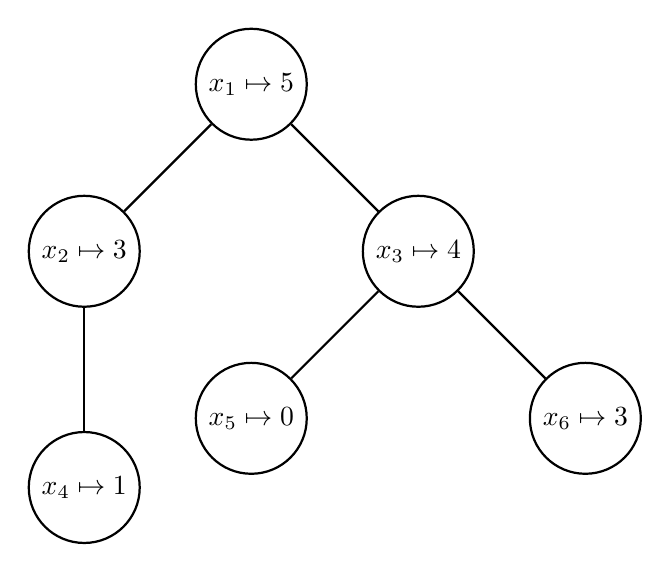
\begin{tikzpicture}[node distance={30mm}, thick, main/.style = {draw, circle}] 
\node[main] (1) {$x_1\mapsto 5$}; 
\node[main] (2) [below left of=1] {$x_2\mapsto 3$}; 
\node[main] (3) [below right of=1] {$x_3\mapsto 4$}; 
\node[main] (4) [below of=2] {$x_4\mapsto 1$}; 
\node[main] (5) [below left of=3] {$x_5\mapsto 0$}; 
\node[main] (6) [below right of=3] {$x_6\mapsto 3$}; 
\draw (1) -- (2); 
\draw (1) -- (3); 
\draw (2) -- (4); 
\draw (3) -- (5); 
\draw (3) -- (6); 
\end{tikzpicture} 

\end{center}

Then $\omega^-(x_1)=x_4$. So $\omega$ maps 
to local minimums, but not necessarily to absolute ones,
even when restricting to the same component. 


\end{example}



